\section{Basic Clojure, Java and JVM Language performance}

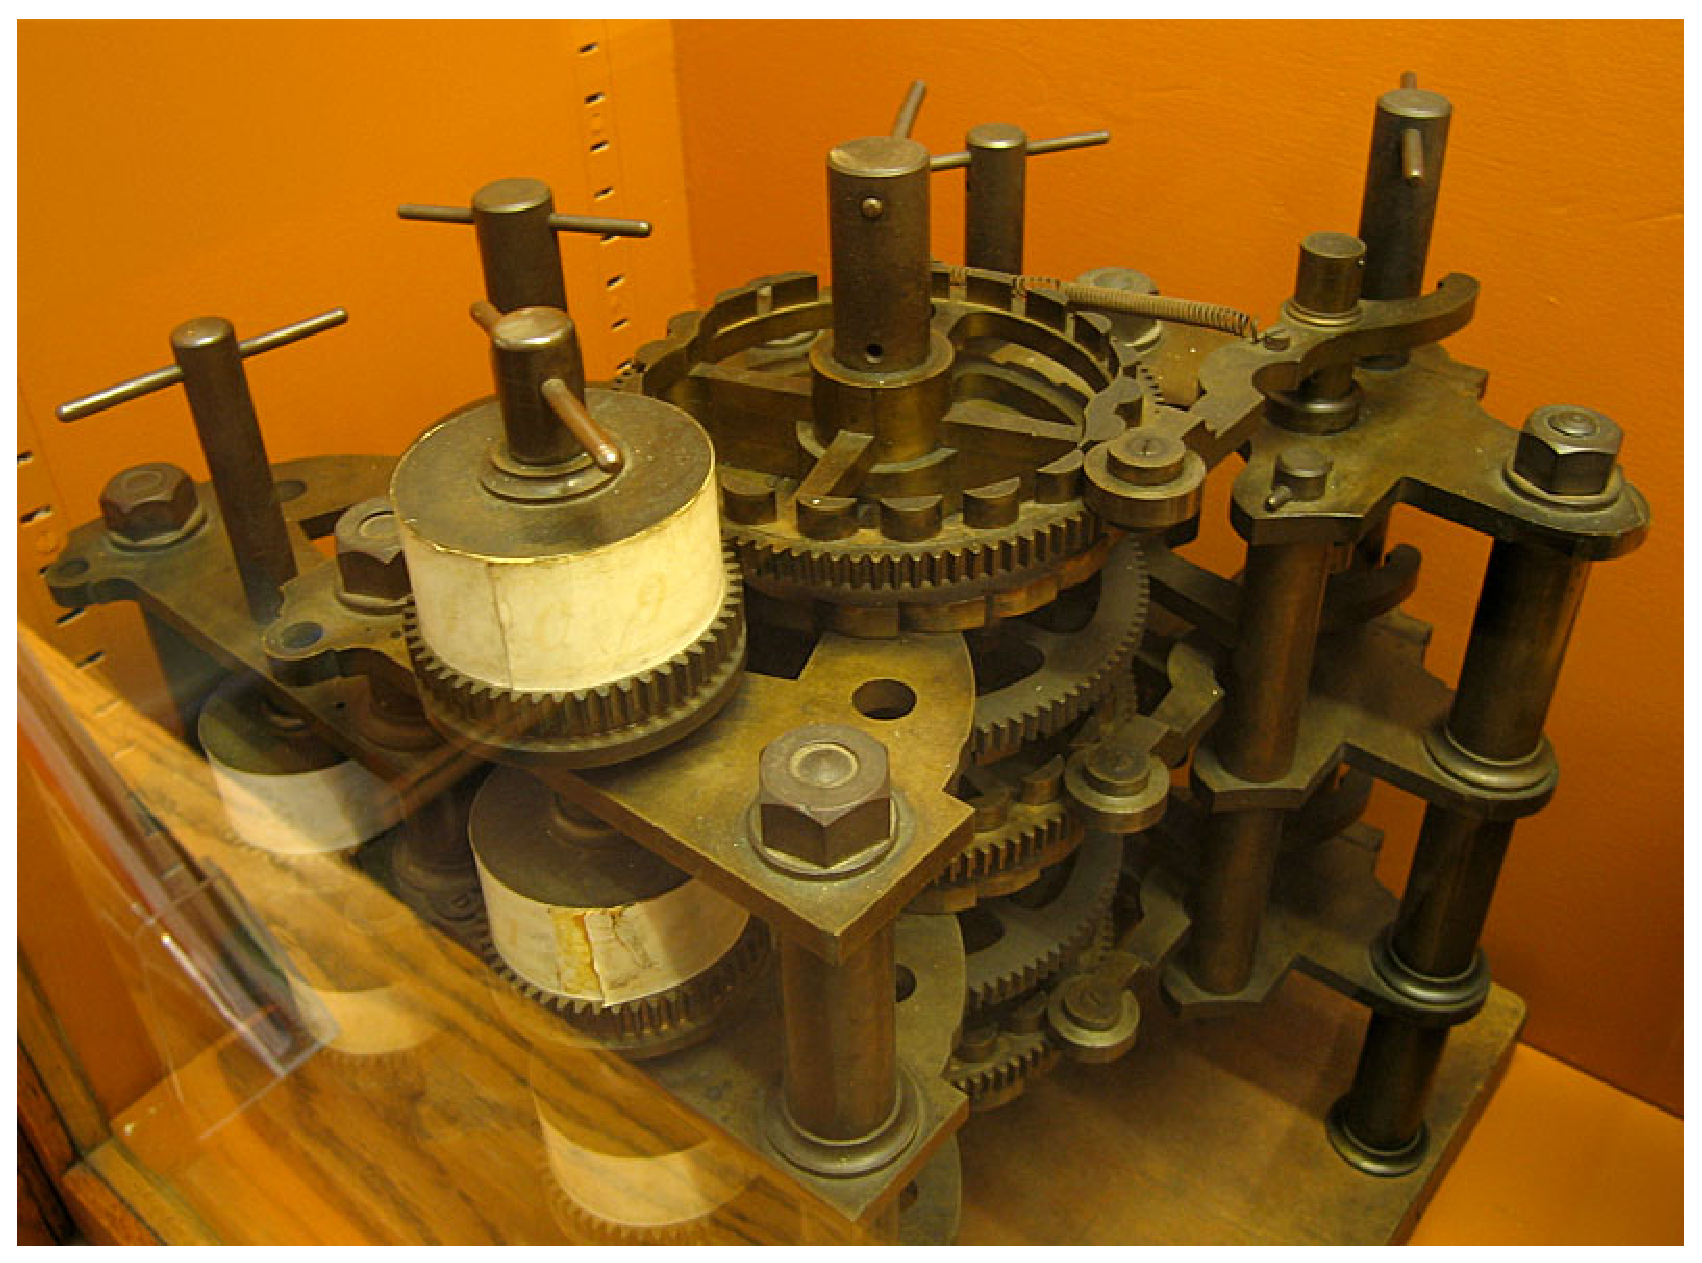
\includegraphics[width=110mm]{BabbageDifferenceEngine.eps}

"Measure, don't guess. The primary goal of all performance tuning exercises should be maximize the end user experience given the resource constraints."

"It isn't so much a "farewell to the J" as an expansion of the platform opportunities Java provides. Sun's investment to power ongoing development of JRuby and Jython broadens the range and reach of Java, as a whole." -- Rick Ross

\subsection{Overview and JVM Languages}

One of the exciting trends to recently emerge from the Java community is the concept of the JVM language. These technologies are all that you would expect them to be. They are implementations of languages that run on the Java Virtual Machine. Some are newly created and some are based on existing, more mature languages. JRuby, Jython are two JVM languages based on CRuby and CPython. Groovy, Scala, Clojure are three completely new JVM languages that were created to add new language features that weren't supported by the core Java language. Some must or can be compiled. Some run without compilation. You can easily compile Scala code to Java bytecode. Clojure also allows this feature (ahead of time compilation). Clojure and JRuby code can also run without having be explicitly compiled. You can interact with the language. In most cases and with most JVM languages, you have full access to existing libraries that were written in pure Java. And normally you can access existing JVM language code from Java (known as Java interoperability). In most cases, it is easier to access Java calls from the JVM language than it is to call the language code from Java. It really depends on the language. In the snippet below, there is a call to the System static method, 'nanoTime'. Simply invoke the system like you would from pure Java.

\begin{verbatim}
require 'java'

def helloWorldBaseline
  # Run the application
  start1 = java.lang.System.nanoTime()
  arr = Array.new
  (1..1000000).each {
    res = 2.2 * 4.1 * 5.4
  }
  end1 = java.lang.System.nanoTime()
  diff = (end1 - start1) * 1e-6  
  puts "Elapsed Time: #{diff} ms"
end
\end{verbatim}

On Dynamic Compilation - "Clojure is a compiled language, so one might wonder when you have to run the compiler. You don't. Anything you enter into the REPL or load using load-file is automatically compiled to JVM bytecode on the fly. Compiling ahead-of-time is also possible, but not required" -- Clojure Docs on being Dynamic.

\subsection{JVM Performance}

"If you want to measure something, then don’t measure other shit." -- Zed Shaw

For the more popular JVM languages, like JRuby and Jython, there isn't much of a difference between running code in their respective C implementations. JRuby is especially well known for being very portable. With JRuby release 1.3.1, JRuby is compatible with CRuby 1.8.6. Jython 2.5.0 was released last month and brings the level of compatibility to CPython versions 2.5. Django and other popular CPython based frameworks are able to work with Jython. You may be wondering, if the Java Virtual Machine language is compatible with the C language, native implementation, is there a loss in performance when running on the Java Virtual Machine? Is there a major loss in performance? That is this purpose of this document, how much time does it take for a particular piece of code to run in JVM language? How long does it take to run similar routines using pure Java code? I want to make it clear, you will not find a large scientific benchmark run under clean room like conditions. I want to present a simple set of routines and how long it took to run. How long did the Clojure code run? How long did the Scala code run? Basically, I want to present the code and how long each test ran, but I don't want to claim that anyone language or piece of code is faster or slower based on these tests. You could say that most of the pure Java code ran faster. Most of the time, that is what happened after running these tests. But there is too much confounding in my tests. Like Zed Shaw said, "If you want to measure something, then don't measure other shit." [3] There is a lot of stuff in my tests to not make these an official comparison. There is a lot of confounding. But, here is the code, here is how long it took to run? It be relevant in more common tests like a Project Euler problem. Project Euler is a website that contains math problems intended to be solved with computer programs. In Project Euler problem number one, I write a program in Clojure and then in Java. They both run on the JVM and the same value is returned. What was the execution time for each program? Simple tests, simple results.

When working with JVM languages and possible performance bottlenecks, you want to consider execution time, but you also want to look at the garbage collector and heap memory usage. Garbage collection is an expensive operation. It won't take a minute to run a garbage collect, but it will take cpu cycles away from your application. JVM code runs in a protected environment, the garbage collector provides automatic memory management and normally protects you from improper memory use. And the garbage collector attempts to free up memory that is no longer needed. You can't normally control when the JVM runs garbage collection and certainly don't want force it. But if you monitor your application, you can identify memory leaks or other problems that might cause performance bottlenecks. It will normally be evident where there is a problem. If you see too many garbage collects within a very short period of time and your total available memory is maxed out, you might eventually encounter an out of memory error. In a long running server environment, most of your performance issues might be alleviated if you look at proper heap memory use. Is your code forcing too many garbage collections within a short period of time? Are you creating too many large objects and holding on to them for too long? In performance tuning your application, there are many things to consider. It may not just be improving a particular algorithm. Consider heap memory and object allocation as well. For most of the tests, there are performance stats, memory stats and other garbage collection statistics.

\subsection{On Clojure}

Clojure is a Lisp dialect created in 2007 by Rich Hickey. It recently reached a 1.0 release and has a large following of Java programmers and Common Lisp developers. Since the Dec 2008 release, the Clojure library has received 18,000 downloads (based on Google Code Stats). Clojure is a dynamically (dynamic/strong) typed language, supports lazy sequences, immutable data structures, macros, and functions as first class objects [4]. Clojure is a functional language just like Common Lisp is a functional language. It is a Lisp dialect so that includes the fully parenthesized syntax. Most syntax will include a function or macro call with arguments or no arguments enclosed by a left and right parenthesis.

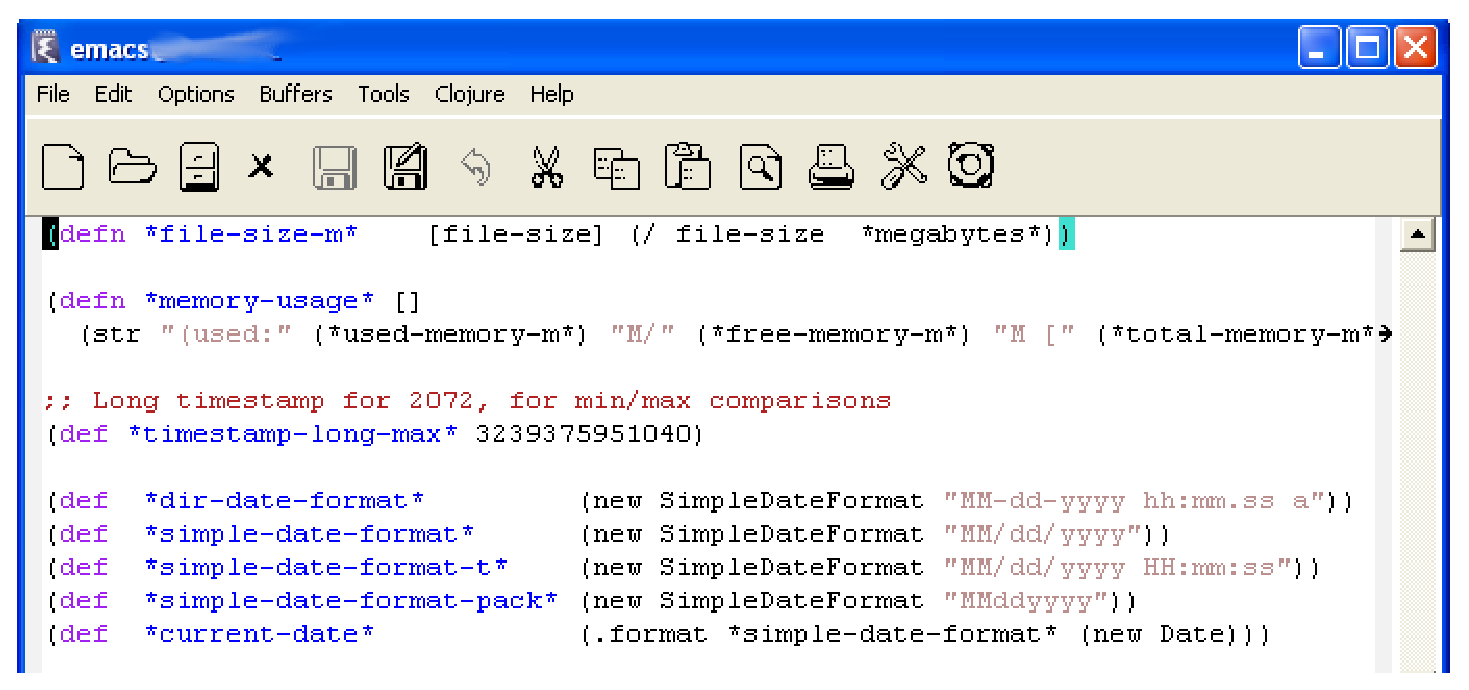
\includegraphics[width=110mm]{emacs_2.eps}

\subsection{Syntax}

Most newcomers to a Lisp dialect may get distracted by the parentheses, the symbolic expressions. They can seem daunting if you are more familiar to a language like C++ or Java. But, this actually is one of the major benefits of Lisp. The simple syntax, functional call, args very much resemble how the compiler or parser will interpret the code. Simple is good. Simple is fast, especially to the machine. It can also benefit the developer because you aren't overburdened with a bunch of syntax to memorize.

It also really helps to have a great editor like Emacs. Emacs is built with its own Lisp dialect, Emacs Lisp. So, Clojure syntax is not too foreign to Emacs. You will need to download the Clojure Emacs Mode and you want to add Slime integration.

Here is a snippet of Clojure code. Just focus on the left parenthesis and the token adjacent to the character. The token, function or macro call and the left parenthesis.

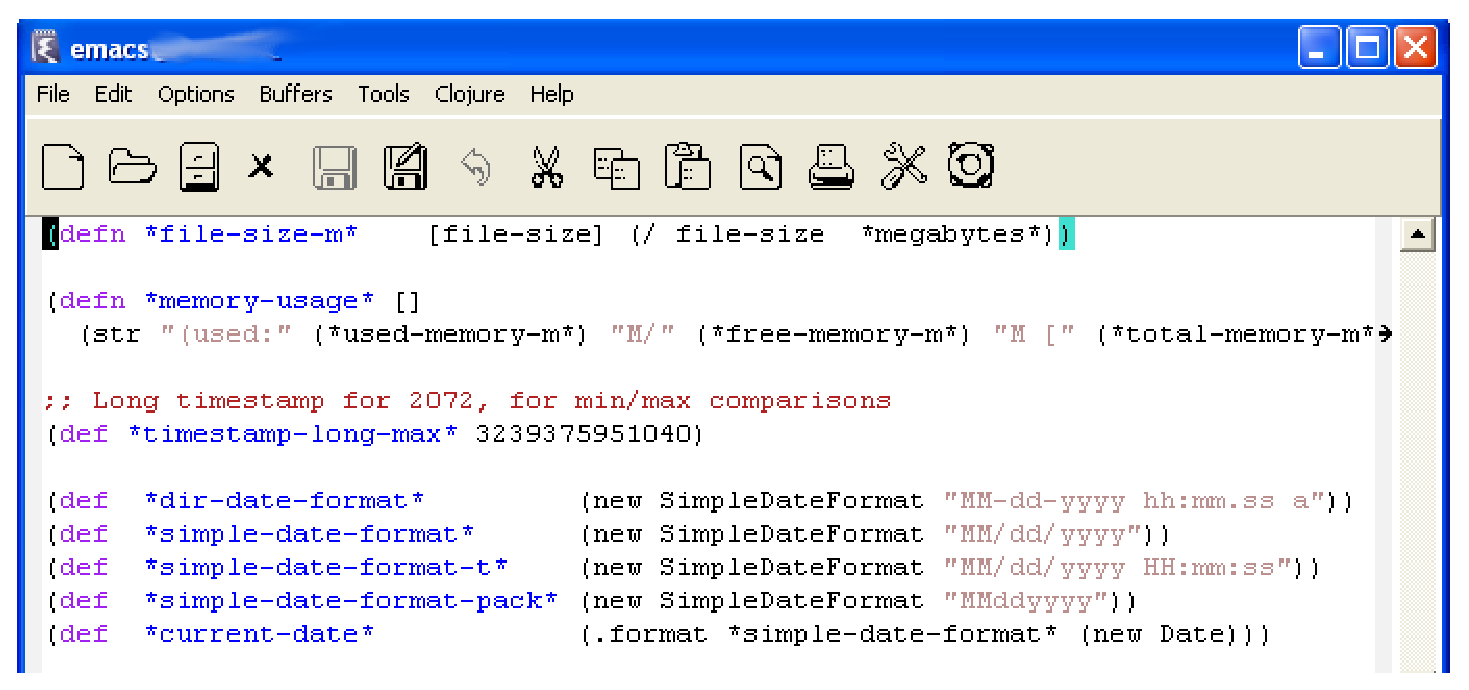
\includegraphics[width=110mm]{emacs_2.eps}

Lisp does not normally get more complicated than the parenthesis tokens and defining function bodies. A function/macro call and arguments. The arguments are normally separated by a variable number of spaces and may include calling another routine. That is the essence of functional programming. You have functions that return some value and can call other functions. You don't have to worry about Object creation syntax, for loop syntax, anonymous inner classes or things that you might encounter with Java. Here is some sample Java code. Look at all the tokens that part of the language.

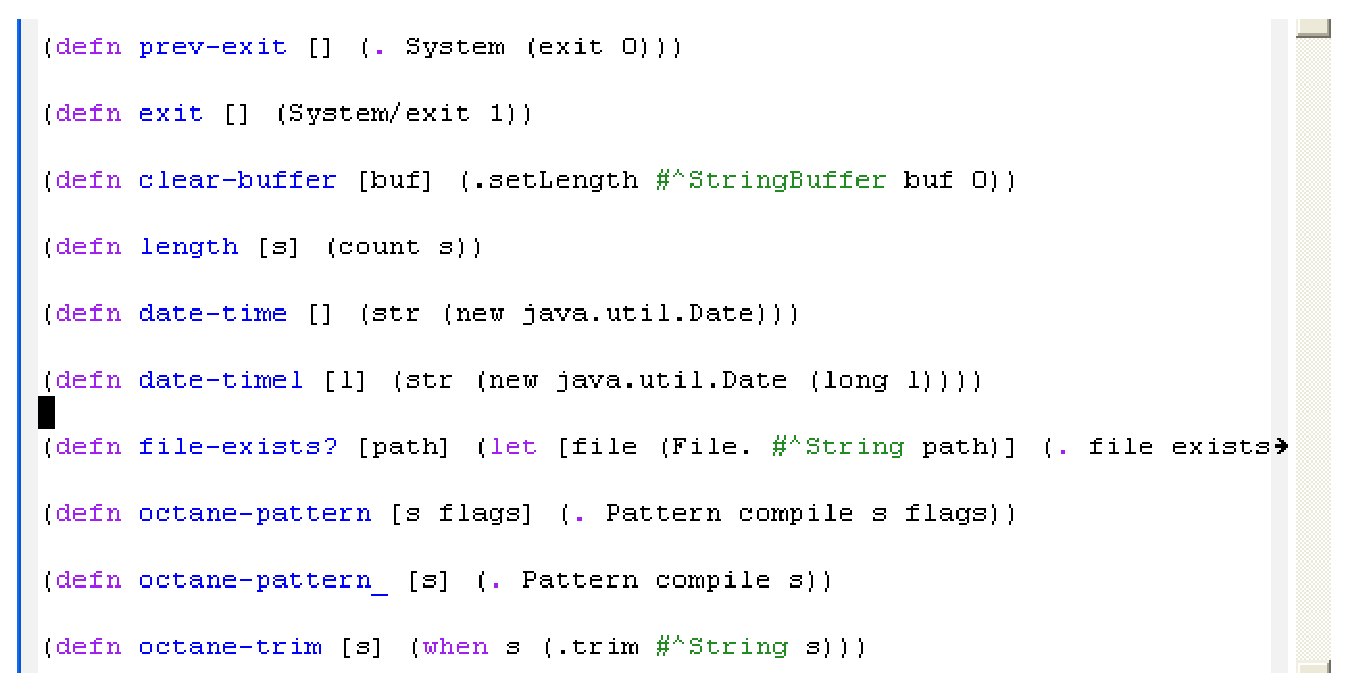
\includegraphics[width=110mm]{lisp_3.eps}

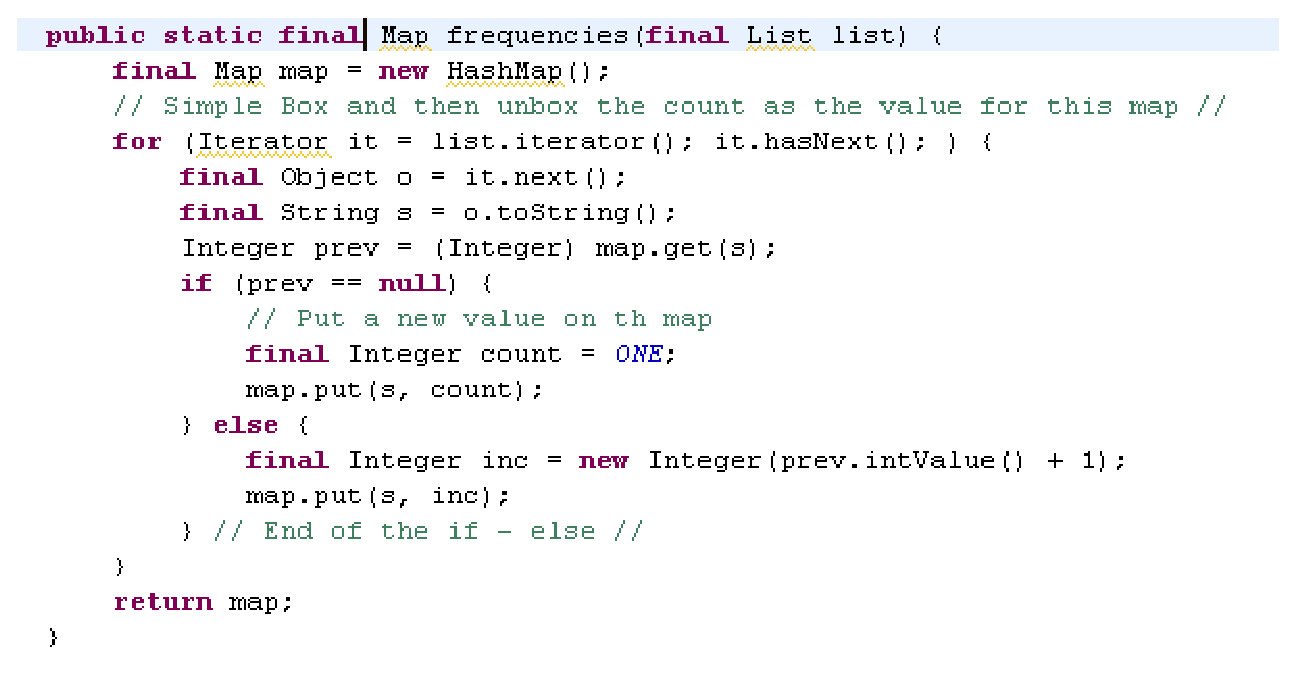
\includegraphics[width=110mm]{java_4.eps}

Note: With this document, I tried not to position one language as better or worse than the other. Each technology that I mention has advantages and disadvantages for writing software. Each tool may give the developer productivity gains and some developers may never get used to changing to a new syntax, never truly realizing some of the intended benefits that the language has to offer. You will have to evaluate these languages (or not) on your own and make. I merely try to point out some of the similarities and some of the differences.

Lisp certainly suffers from that old adage, "easy to learn, may take a lifetime to master". It is easy to write Lisp code, it may take time to write readable, solid, idiomatic Lisp code. I am sure I will get many comments on how to write more idiomatic Clojure code even for these rudimentary examples. Luckily, Clojure has many of the functions that you will encounter with most other Lisp dialects. In Java or C++, you may be accustomed to the 'for loop' syntax. Here is the Clojure macro for building a list of elements.

'For' Clojure API Documentation: "List comprehension. Takes a vector of one or more binding-form/collection-expr pairs, each followed by zero or more modifiers, and yields a lazy sequence of evaluations of expr. Collections are iterated in a nested fashion, rightmost fastest, and nested coll-exprs can refer to bindings created in prior binding-forms."

\begin{verbatim}
;; Macro definition for 'for'
(defmacro for
  [seq-exprs body-expr]
  (assert-args for
     (vector? seq-exprs) "a vector for its binding"
     (even? (count seq-exprs)) "an even number of forms in binding vector")
  (let [to-groups (fn [seq-exprs]
                      (reduce (fn [groups [k v]]
                              (if (keyword? k)
                                (conj (pop groups) (conj (peek groups) [k v]))
                                (conj groups [k v])))
                              [] (partition 2 seq-exprs)))
        err (fn [& msg] (throw (IllegalArgumentException. (apply str msg))))
        emit-bind (fn emit-bind [[[bind expr & mod-pairs]
                                  & [[_ next-expr] :as next-groups]]]
                      (let [giter (gensym "iter__")
                            gxs (gensym "s__")
                            do-mod (fn do-mod [[[k v :as pair] & etc]]
                                       (cond
                                        (= k :let) `(let ~v ~(do-mod etc))
                                        (= k :while) `(when ~v ~(do-mod etc))
                                        (= k :when) `(if ~v
                                                       ~(do-mod etc)
                                                       (recur (rest ~gxs)))
                                        (keyword? k) (err "Invalid 'for' keyword " k)
                                        next-groups
                                        `(let [iterys# ~(emit-bind next-groups)
                                               fs# (seq (iterys# ~next-expr))]
                                           (if fs#
                                             (concat fs# (~giter (rest ~gxs)))
                                             (recur (rest ~gxs))))
                                     :else `(cons ~body-expr
                                                  (~giter (rest ~gxs)))))]
                        `(fn ~giter [~gxs]
                         (lazy-seq
                          (loop [~gxs ~gxs]
                            (when-first [~bind ~gxs]
                                        ~(do-mod mod-pairs)))))))]
    `(let [iter# ~(emit-bind (to-groups seq-exprs))]
       (iter# ~(second seq-exprs)))))
;; END OF MACRO (code from core.clj, clojure source);;
\end{verbatim}

OK, that was a little daunting, but it is good to know the code for all of the Clojure source is freely available. This a yet another added benefit that you may not capitalize on, but all of the Clojure source is highly readable and lightweight. There are only 24k lines of Java code in the clojure.lang package. And only 7k lines of Clojure source in the core libray. I routinely make changes to the Clojure Java code to add trace logic. It took only 10 minutes to figure out where I needed to place my logic and then compile with my own Ant script. Imagine making similar changes to the Java API?

\subsection{More on the Clojure, Java source for the performance tests}

I used a simple format for the performance tests that I will present later in the document. I wrote or used existing code from a third-party and then ran the code. There may be many differences between the style of code. And the Clojure code may not be idiomatic. But it should be close. Here is the source for the Quick Sort, Clojure and Java:

\begin{verbatim}
;; Two versions of the Clojure Quick Sort:
(defn qsort 
  "Quick sort from rosetta code:
 http://rosettacode.org/wiki/Quicksort#Clojure"
  [[pvt & rs]]
  (if pvt
    `(~@(qsort (filter #(<  % pvt) rs))
      ~pvt 
      ~@(qsort (filter #(>= % pvt) rs)))))

(defn qsort-2 [[pivot & xs]]
  (when pivot
    (let [smaller #(< % pivot)]
      (lazy-cat (qsort-2 (filter smaller xs))
                [pivot]
                (qsort-2 (remove smaller xs))))))

(dotimes [x 4]
      (println "i: " (int (Math/pow 10.0 x)))
    (time (count (qsort (for [_ (range (int (Math/pow 10.0 x))) ] 
                          (.nextInt random))))))



// JAVA VERSION OF QUICK SORT
    public static final List quicksort(final List arr) {
        if (arr.size() <= 1) {
            return arr;
        }
        Integer pivot = (Integer) arr.get(0);
     
        List less = new LinkedList();
        List pivotList = new LinkedList();
        List more = new LinkedList();
     
        // Partition
        for (Iterator it = arr.iterator(); it.hasNext();) {
            Integer i = (Integer) it.next();
            if (i.compareTo(pivot) < 0) {
                less.add(i);
            } else if (i.compareTo(pivot) > 0) {
                more.add(i);
            } else {
                pivotList.add(i);
            } // End of the if - else //
            
        } // End of the for //
     
        // Recursively sort sublists
        less = quicksort(less);
        more = quicksort(more);
     
        // Concatenate results
        less.addAll(pivotList);
        less.addAll(more);
        return less;
    }
// END OF EXAMPLE 
\end{verbatim}

\subsection{Performance Results}

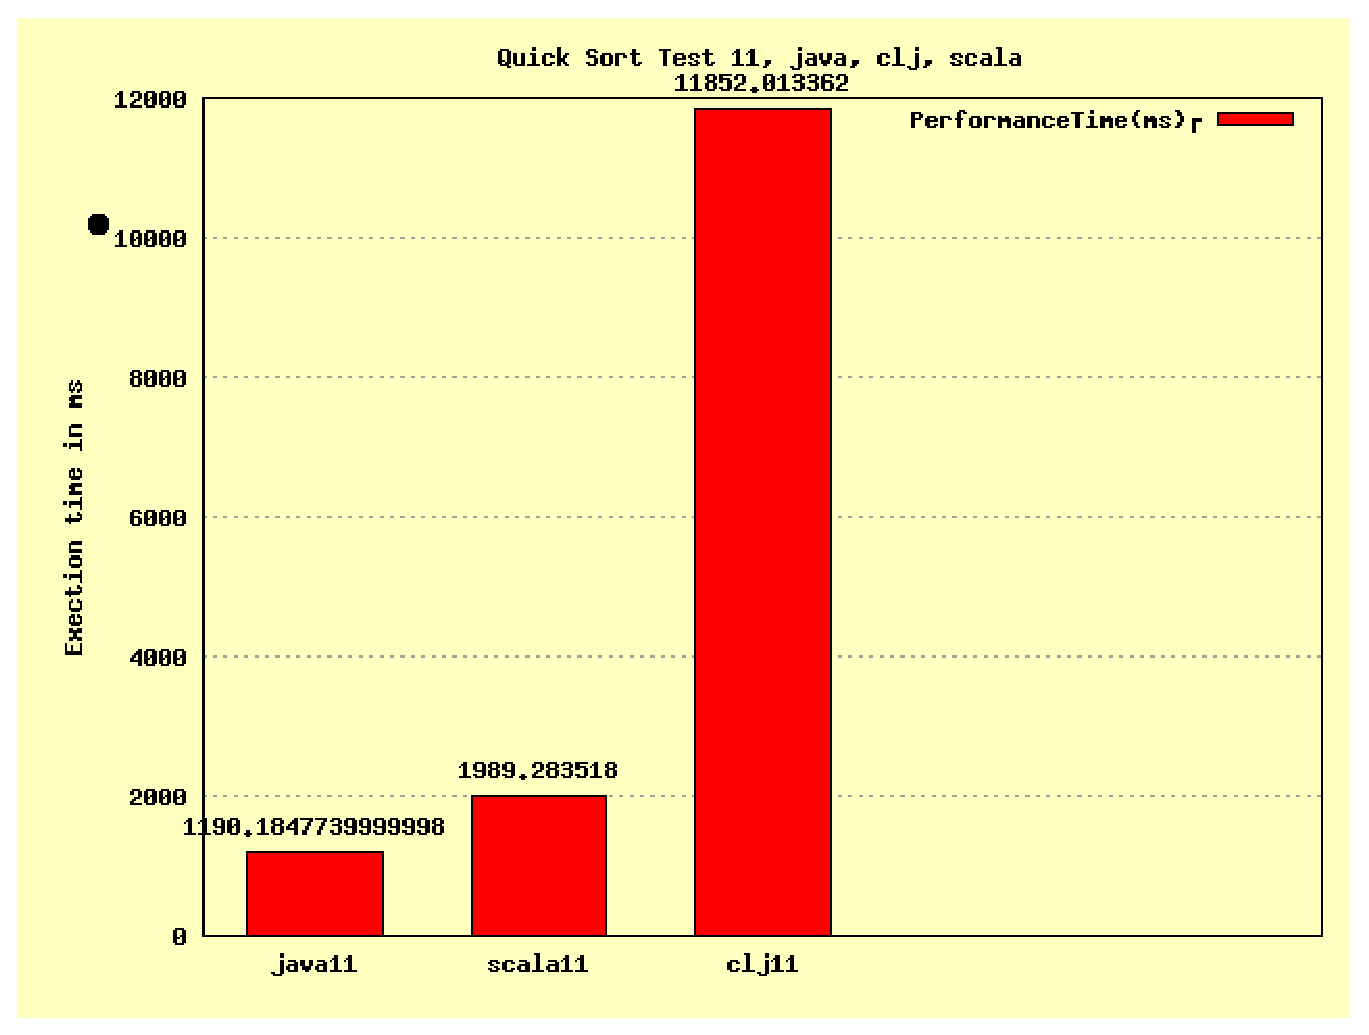
\includegraphics[width=110mm]{chart1_scala_8.eps}
\begin{verbatim}
JavaTest   PerformanceTime(ms)
#####      ########### 
java11     1190.1847739999998              
jruby11    5068.168914            
clj11      11852.013362
\end{verbatim}

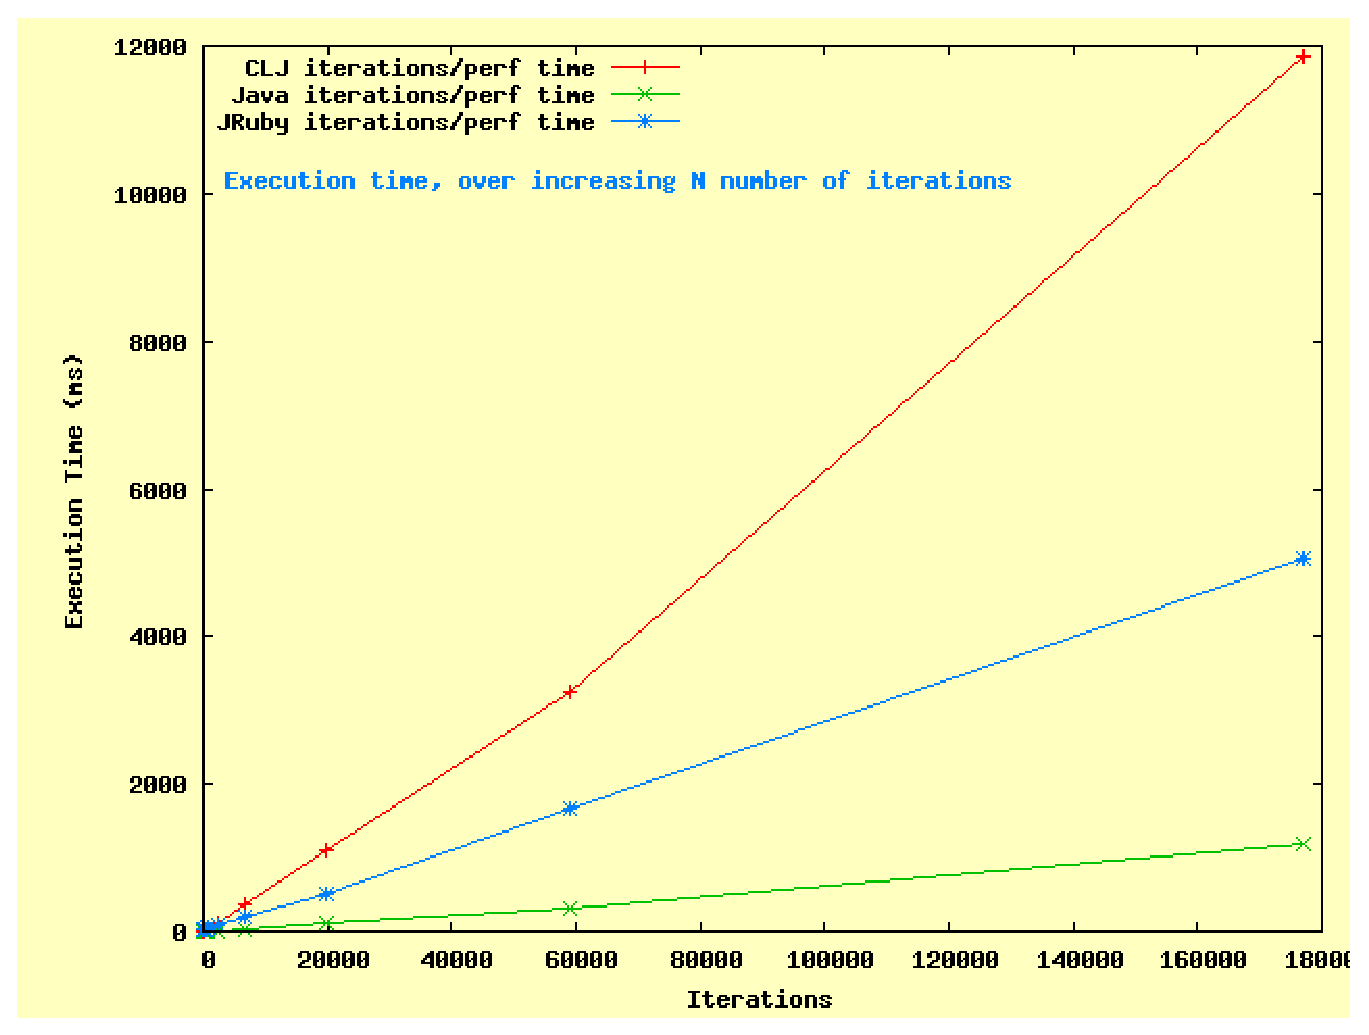
\includegraphics[width=110mm]{line_clj_sort_6.eps}

\subsection{JRuby and Scala Source, Scala Performance for the Simple Quick Sort}

Scala was created in 2001 and is currently at version 2.7.5 as of 6/3/2009. Scala is a stark contrast to Clojure. David Pollak had this to say about Scala's type system, "Put another way, Scala is statically typed with optional duck typing... the opposite of Objective-C et. al. with their duck typing with optional static typing." Clojure on the other hand is dynamic in the sense that you don't have to explicitly define a type whenever you need to use a particular object, but you can define the type specification using type hints.

\begin{verbatim}
;; Notice, second version uses the String type hint
(defn str-split-refl [s regex]
      (vec (. s split regex)))
(defn str-split-fast [#^String s regex]
      (vec (. s split regex)))
\end{verbatim}

The above example presents two versions of a string split method, in Clojure. The second version use the String type hint to help the compiler determine the type for future calls in that function. On Scala's type system, "Scala is equipped with an expressive type system that enforces statically that abstractions are used in a safe and coherent manner"

\subsection{When would you use a JVM language? (Scala, Clojure, or just Java)}

Why even investigate a JVM language? What is the point? A programming language is like any other tool or library used to create and interact with other software or hardware components? If you work in a web or J2EE environment, you might write SQL code, define CSS scripts, write Javascript code, write HTML/XHTML. It isn't uncommon for web application developers to write Java, sql, css, javascript or HTML code. Sometimes all within the same day, sometimes during different phases of a project. That doesn't take into account the number libraries that you must normally learn, understand and work with. So, NOT learning a new JVM programming language just on the premise that it is something different, isn't a valid reason for not using it. People have asked me, would you use Clojure, Java, or Scala? I have used all three for small GUI projects. I have used Scala for the the backend API where I don't need to make small changes. I used Clojure because of the dynamic nature of the language. I can make many, quick incremental changes without having any major impact on the Scala backend API. Take the Java api for example. Most of the core library is set in stone. The java.lang.String class hasn't changed much in over a decade. I see Scala being used for those type of rigid API requirements. This doesn't mean that Clojure couldn't be used for this purpose, it just means that is how I have used Scala and it just seemed to fit because of how easy it is to call Scala from Java (Java interoperability), also because of the nature of Scala's types. Here is just one example on how I used Clojure. The code snippet below contains valid Clojure code used to develop a small GUI application. If you just look at it without understanding the syntax, the code below almost looks like a general purposed configuration file. Here I can easily modify the layout of my GUI window, buttons without ever really getting any complex language details. I am just looking at the data required to change my layout.

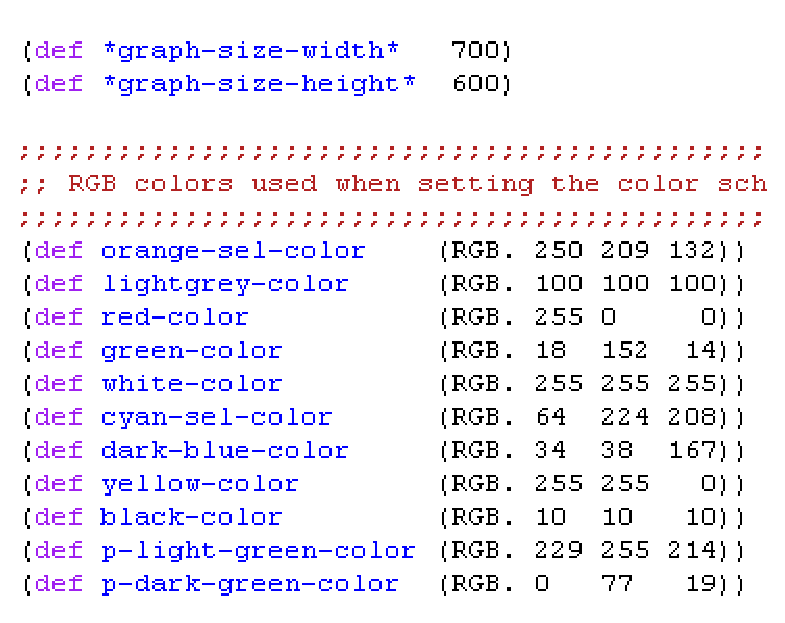
\includegraphics[width=110mm]{easy_clojure_conf_7.eps}

\begin{verbatim}
A blogger from creativekarma.com provided a list of some of Scala's features:

    * Conventional class types,
    * Value class types,
    * Nonnullable types,
    * Monad types,
    * Trait types,
    * Singleton object types (procedural modules, utility classes, etc.),
    * Compound types,
    * Functional types,
    * Case classes,
    * Path-dependent types,
    * Anonymous types,
    * Self types,
    * Type aliases,
    * Generic types,
    * Covariant generic types,
    * Contravariant generic types,
    * Bounded generic types,
    * Abstract types,
    * Existential types,
    * Implicit types,
    * Augmented types,
    * View bounded types, and
    * Structural types which allow a form of duck typing when all else fails.
\end{verbatim}
\begin{verbatim}
// Here is an Example Scala Quick Sort:
 // http://en.literateprograms.org/Quicksort_(Scala)
 // From scala home
  def sort[A <% Ordered[A]](xs: List[A]):List[A] = {
    if (xs.isEmpty || xs.tail.isEmpty) xs
    else {      
      val pivot = xs( xs.length / 2)      
      // list partition
      // initialize boxes
      var lows: List[A] = Nil
      var mids: List[A] = Nil
      var highs: List[A] = Nil      
      for( val item <- xs) {
        // classify item        
        if ( item == pivot) mids = item :: mids
        else if (item < pivot) lows = item :: lows
        else highs = item :: highs
      }
      // return sorted list appending chunks      
      sort(lows) ::: mids ::: sort(highs) 
    }
  }
  // Running the sort and time
  def run(n:Int) = {
    val start1 = java.lang.System.nanoTime()
    //val l = repeat(n)(random.nextInt)
    val l = initialize(n)
    val l2 = sort(l)
    val d = l2.length
    val z = d + 1
    val end1 = java.lang.System.nanoTime()
    val diff = (end1 - start1) * 1e-6
    println("Elapsed Time: " + diff + " ms " + z)
  }
 // End of scala example
\end{verbatim}
\begin{verbatim}
# JRuby Sort Example:
class Array
  def quick_sort
    return self if length <= 1
    pivot = self[length / 2]
    return (find_all { |i| i <  pivot }).quick_sort +
           (find_all { |i| i == pivot }) +
           (find_all { |i| i >  pivot }).quick_sort
  end
end
def runTest1a(n)
  # Run the application
  start1 = java.lang.System.nanoTime()
  arr = Array.new
  (1..n).each {
    arr << rand(100000)
  }
  res = arr.quick_sort
  end1 = java.lang.System.nanoTime()
  diff = (end1 - start1) * 1e-6  
  puts "Elapsed Time: #{diff} ms"
end
# End of Example
\end{verbatim}

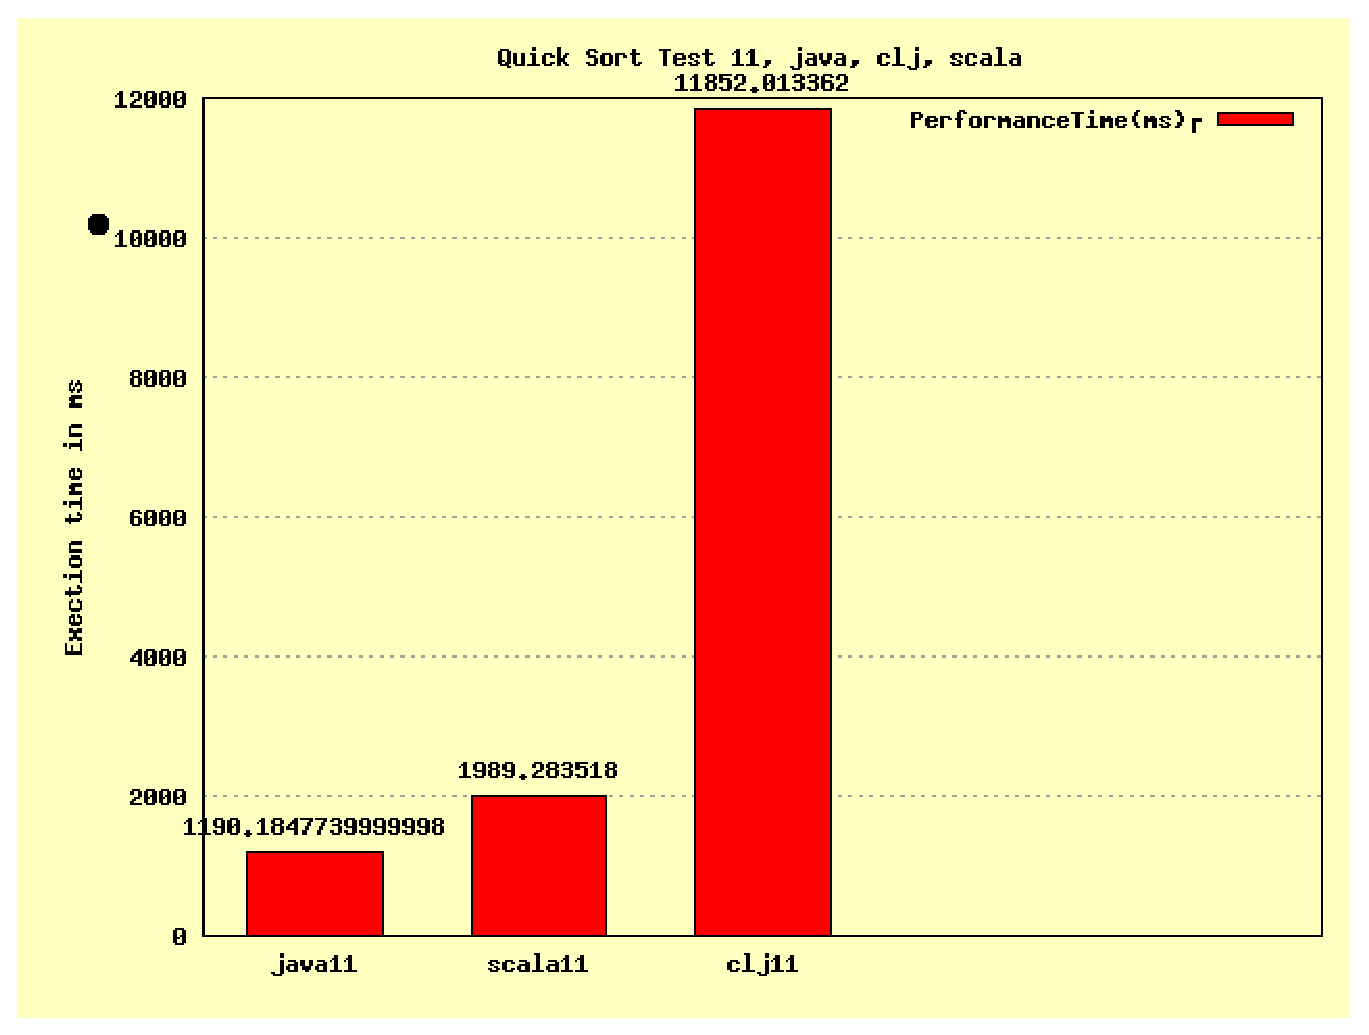
\includegraphics[width=110mm]{chart1_scala_8.eps}
\begin{verbatim}
Test     PerformanceTime(ms)
#####    ########### 
java11   1190.1847739999998              
scala11  1989.283518            
clj11    11852.013362
\end{verbatim}

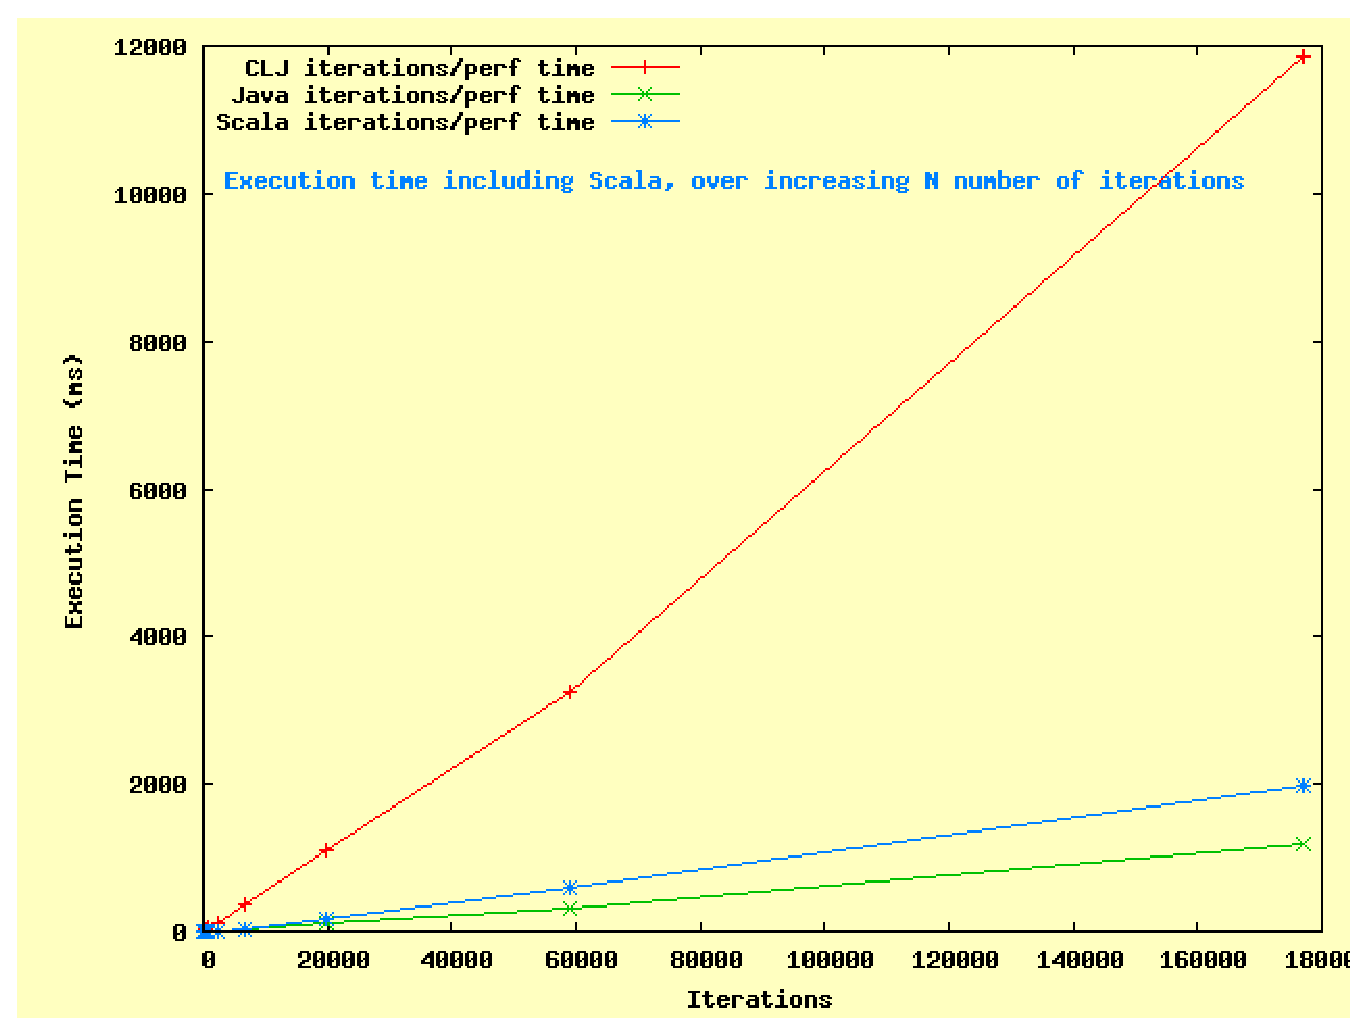
\includegraphics[width=110mm]{line_scala_freq.1__31.eps}

\begin{verbatim}
The line graph is a combination of Java, Scala, and Clojure execution 
times with an increasing number of random elements. 
Here are the results for the Clojure quick sort:

iterat   exectime(ms)
#####    #########
81       8.019583
243      16.82068
729      69.767482
2187     121.894408
6561     370.054832
19683    1096.553958
59049    3245.377605
177147   11852.013362
\end{verbatim}

\subsection{On Garbage Collection}

"If the garbage collector has become a bottleneck, you may wish to customize the generation sizes. Check the verbose garbage collector output, and then explore the sensitivity of your individual performance metric to the garbage collector parameters." -- Tuning Garbage Collection

\begin{verbatim}
Here is some output from the garbage colection report:
...
[GC 1277K->390K(5056K), 0.0006050 secs]
[GC 1286K->399K(5056K), 0.0005540 secs]
[GC 1294K->407K(5056K), 0.0005580 secs]
[GC 1303K->416K(5056K), 0.0009580 secs]
[GC 1311K->424K(5056K), 0.0006540 secs]
[GC 1320K->431K(5056K), 0.0007520 secs]
[GC 1327K->431K(5056K), 0.0012980 secs]
...
...
\end{verbatim}

"With the line below, indicate the combined size of live objects before and after garbage collection, respectively. After minor collections the count includes objects that aren't necessarily alive but can't be reclaimed, either because they are directly alive, or because they are within or referenced from the tenured generation. The number in parenthesis"
\begin{verbatim}
(776768K)(in the first line)
\end{verbatim}
"is the total available space, not counting the space in the permanent generation, which is the total heap minus one of the survivor spaces. The minor collection took about a quarter of a second."

The output is generated with the 'verbosegc' and other JVM options:
(Note: The duplicated 'verbosegc' options gives more information about the garbage collecting)

There are 1400 data points in the output file and in the image for the Clojure sort example. Each GC line in the gc analysis file contains GC information about a minor garbage collection.

"If the incremental collection of the tenured generation cannot be completed before tenured generation is full, a major collection occurs and is indicated in the verbosegc output by the 'MSC' in the output."

Here is the gnuplot representation of the used memory and total available after a minor garbage collection. There were 1400 data points in the clojure test. This is after running the quick sort code above.
\begin{verbatim}
Data Points used in graph:
used after gc | total after gc
...
...
26605 32576
26744 32576
27180 32576
27190 32576
27362 32576
27551 32576
line: 1421 -- 27684 32576
line: 1422 -- 27843 32576
\end{verbatim}

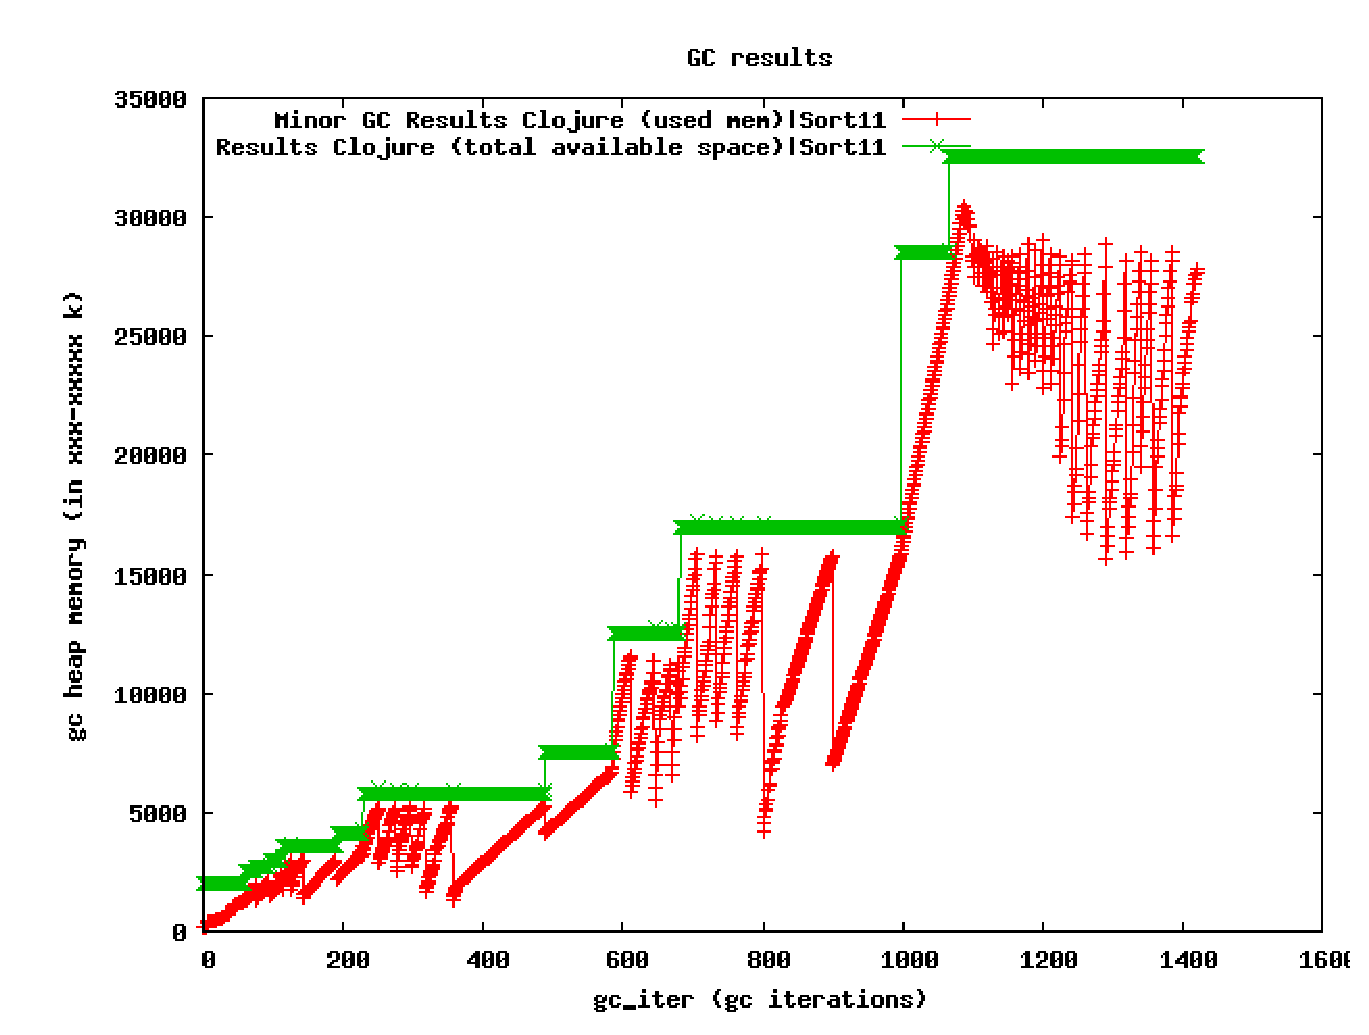
\includegraphics[width=110mm]{gc_1_11_sort_clj_21.eps}

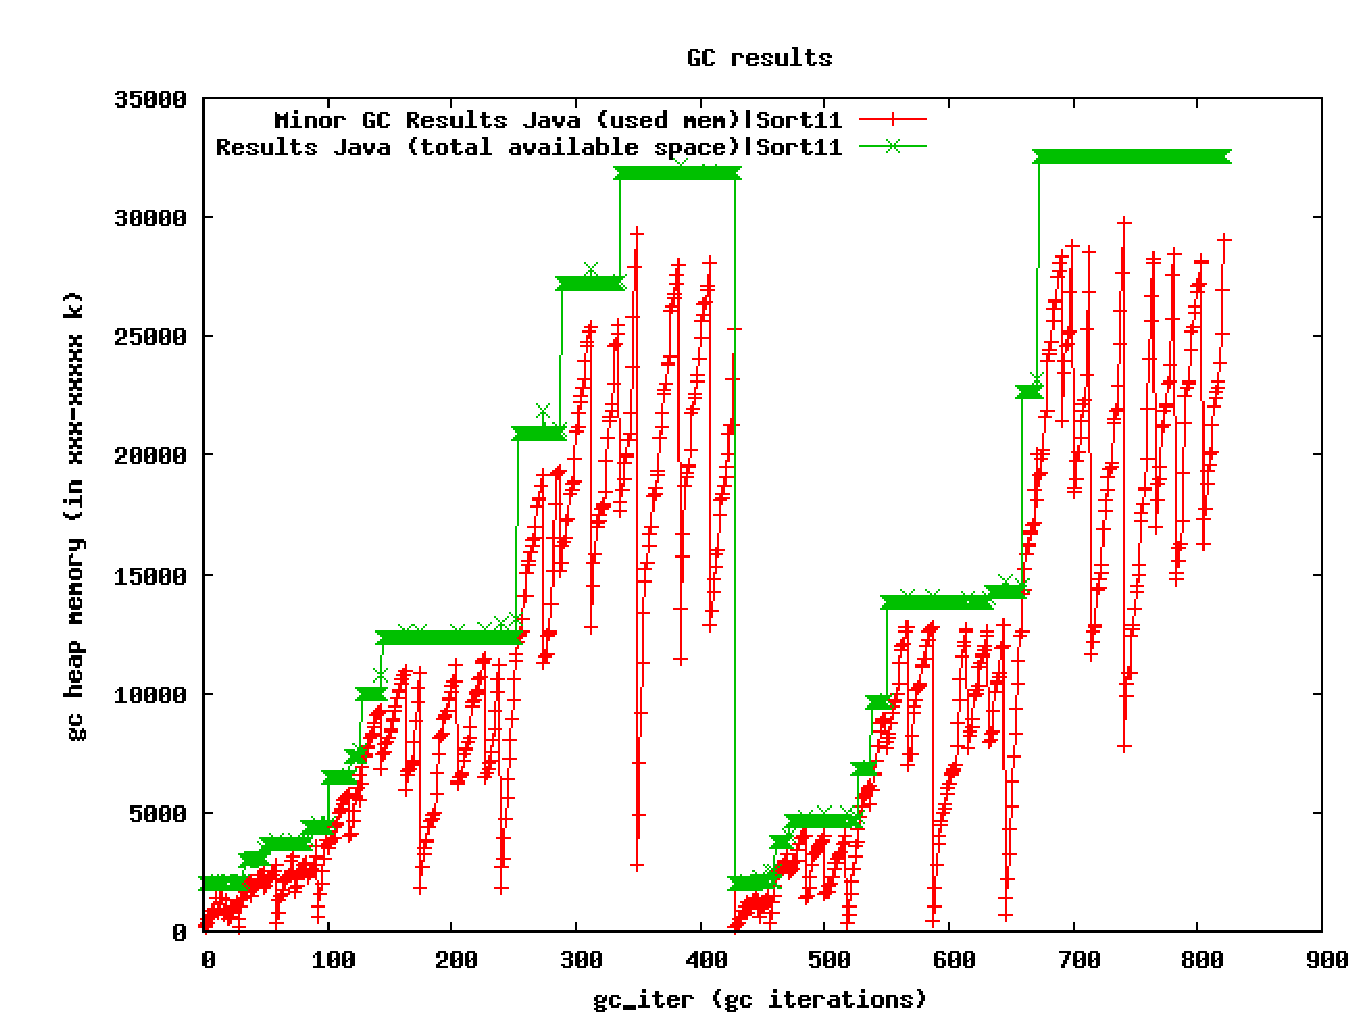
\includegraphics[width=110mm]{gc_2_java_sort_22.eps}

\subsection{Large Objects}

The quick sort example is not a good test to really push the garbage collector. Here is another test, one with Clojure and one with Java. I instantiate a large number of large objects and do the same for small objects. The garbage collector is better at handling smaller objects and consequently not as good at handling large objects (using the default GC rules). So, if you are looking at performance issues, you might look at how often large objects are being created and how long you are holding onto those objects. It is better to create many small objects and retain them for a short time than creating a few number large objects and retaining them for a long time. For example, I guess it is better to write short, static, utility methods and only create objects local to that method. "Large objects might be too big for Eden and will go directly to the old generation area; they will take longer to initialize (when setting fields to their default values such as null and zero); and they might cause fragmentation" [6]. A large object is one that the size of the allocation of the large object within a memory heap exceeds a maximum contiguous free space within the Java heap.


I attempted to create a large object that had many fields with lots of String data. Using my approximate sizeof utility method, it looks like it takes 800kb to create this object.

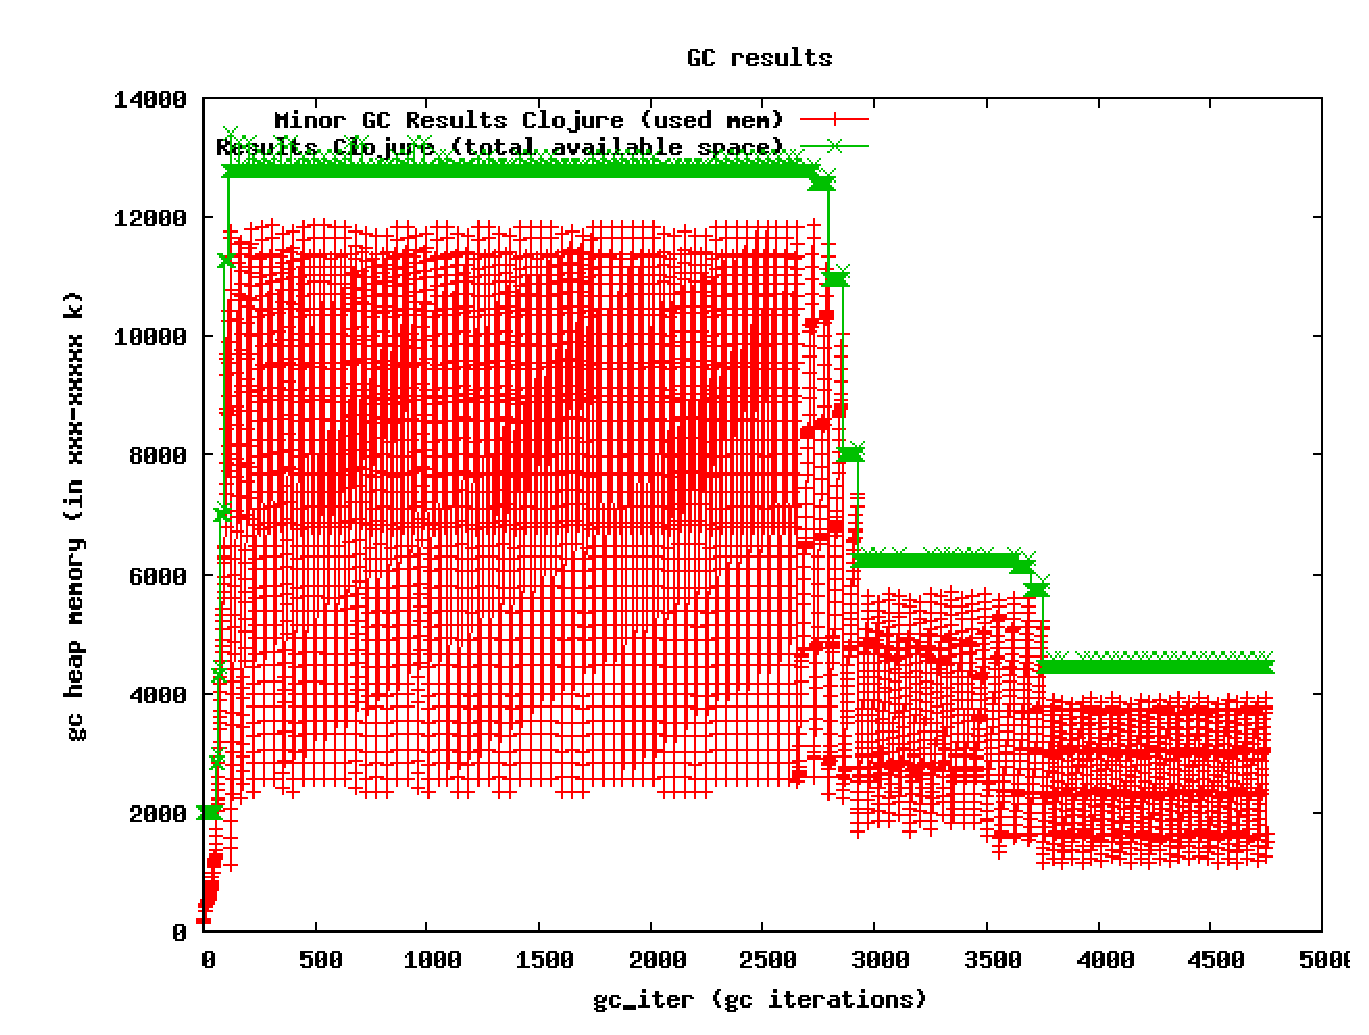
\includegraphics[width=110mm]{gc_5_vars_clj_25.eps}

\subsection{Additional Tools}

There is no shortage of tools for monitoring JVM performance. Mature, open and proprietary monitoring applications are available. Most of them focus garbage collection, heap memory, cpu monitoring, and method trace calls. The netbeans monitor, Sun's jconsole, jrat, and the Eclipse memory analysis tool are a few that I have used recently.

The chart report output from Eclipse's Memory Analysis Tool is depicted below. The overview contains the number of objects, number classes and classloader. The MAT tool also looks at potential memory leaks and the objects that are causing the problem, "biggest consumers" and a heap object histogram. To generate the data, we simply generate a heap dump and open the heap dump file.

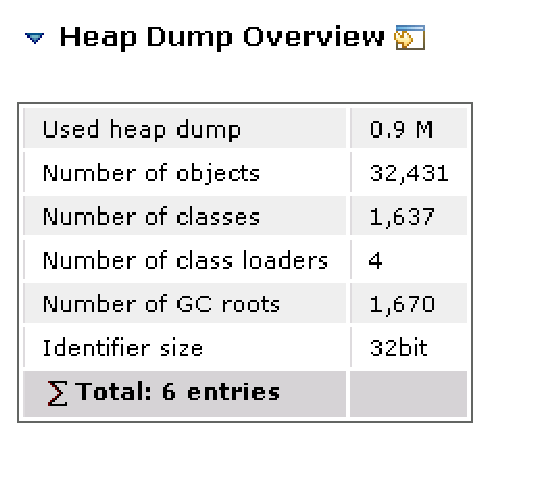
\includegraphics{hist_clj_30.eps}

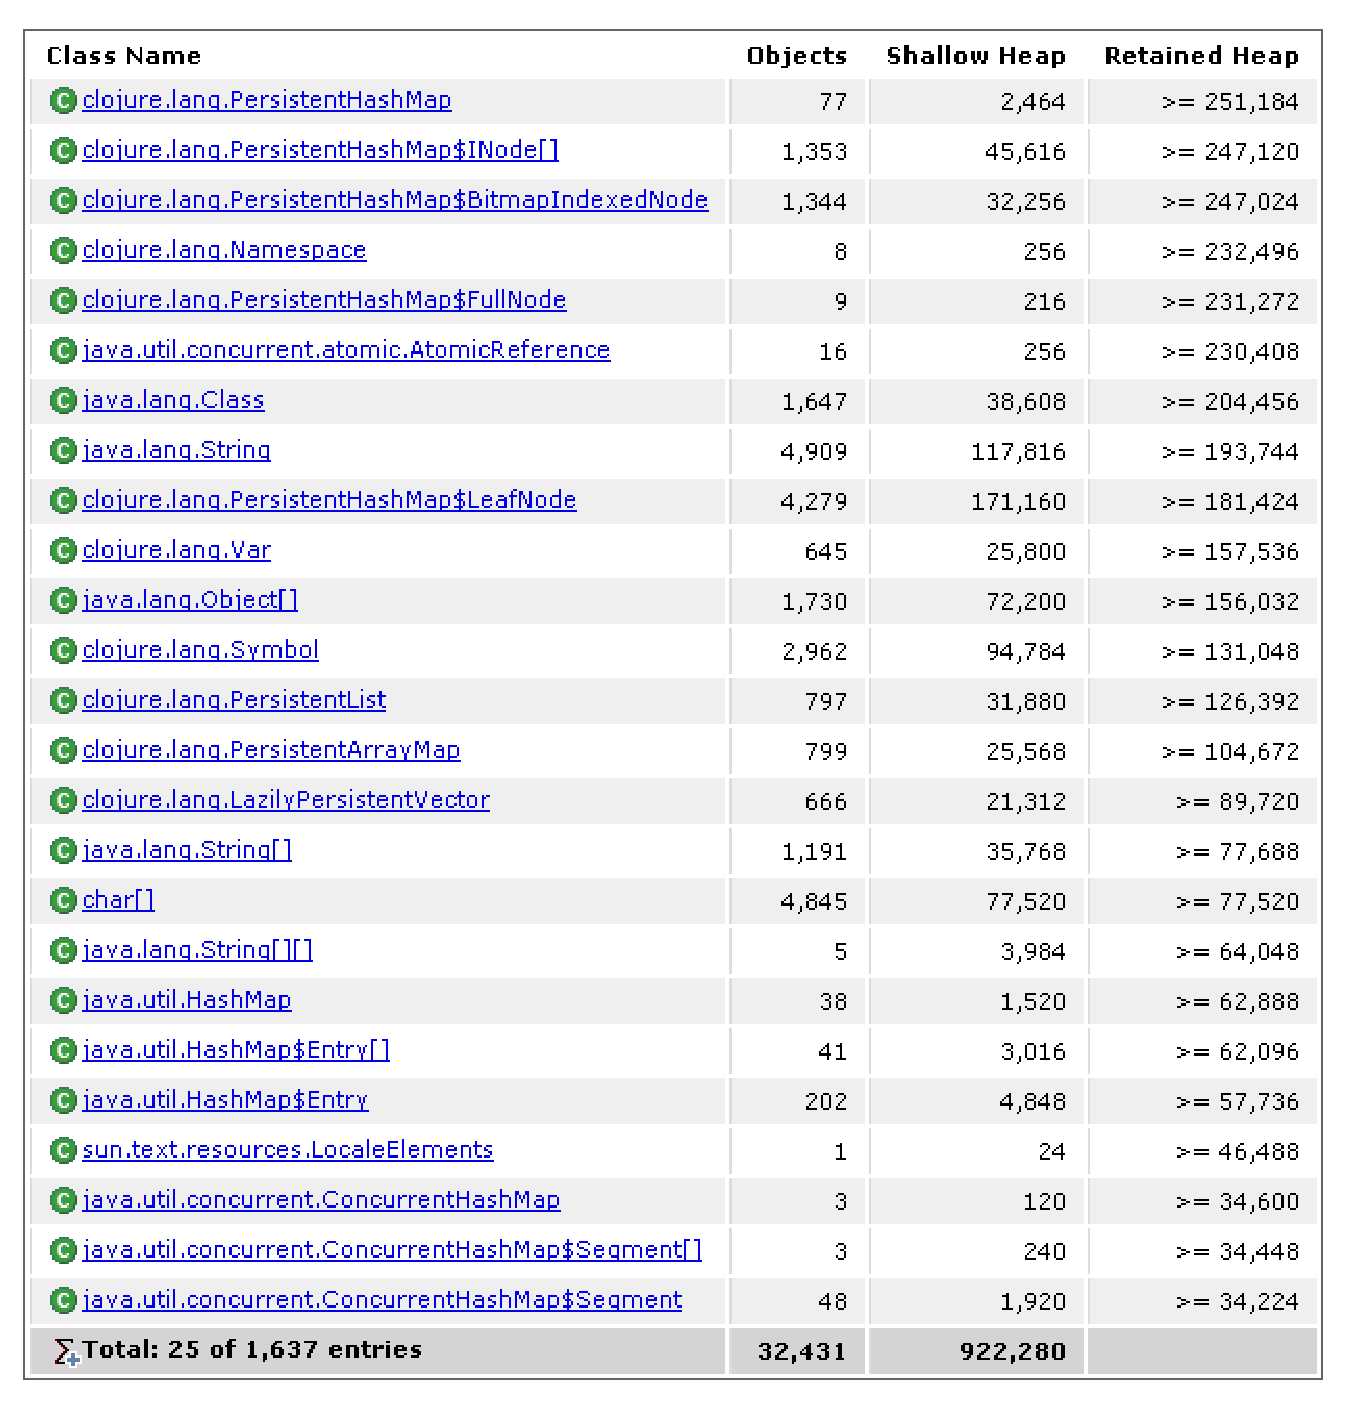
\includegraphics[width=110mm]{mat_hist_31.eps}

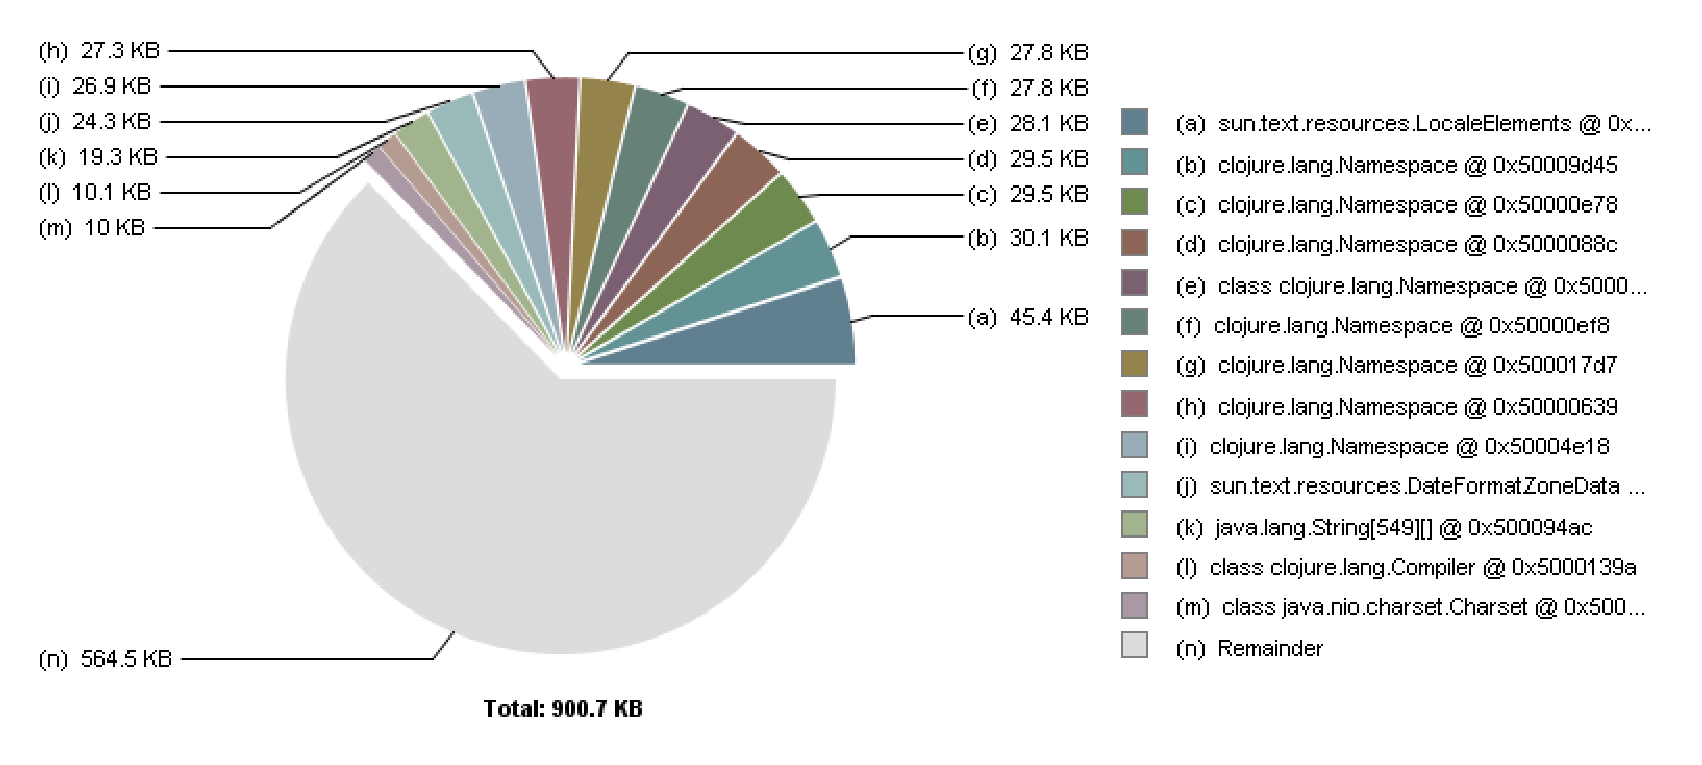
\includegraphics[width=110mm]{map_big_32.eps}

Running JRat or Netbeans profilers is as simple as running with the appropriate JVM args allowing your application to run and then opening the files output after the program has exited.

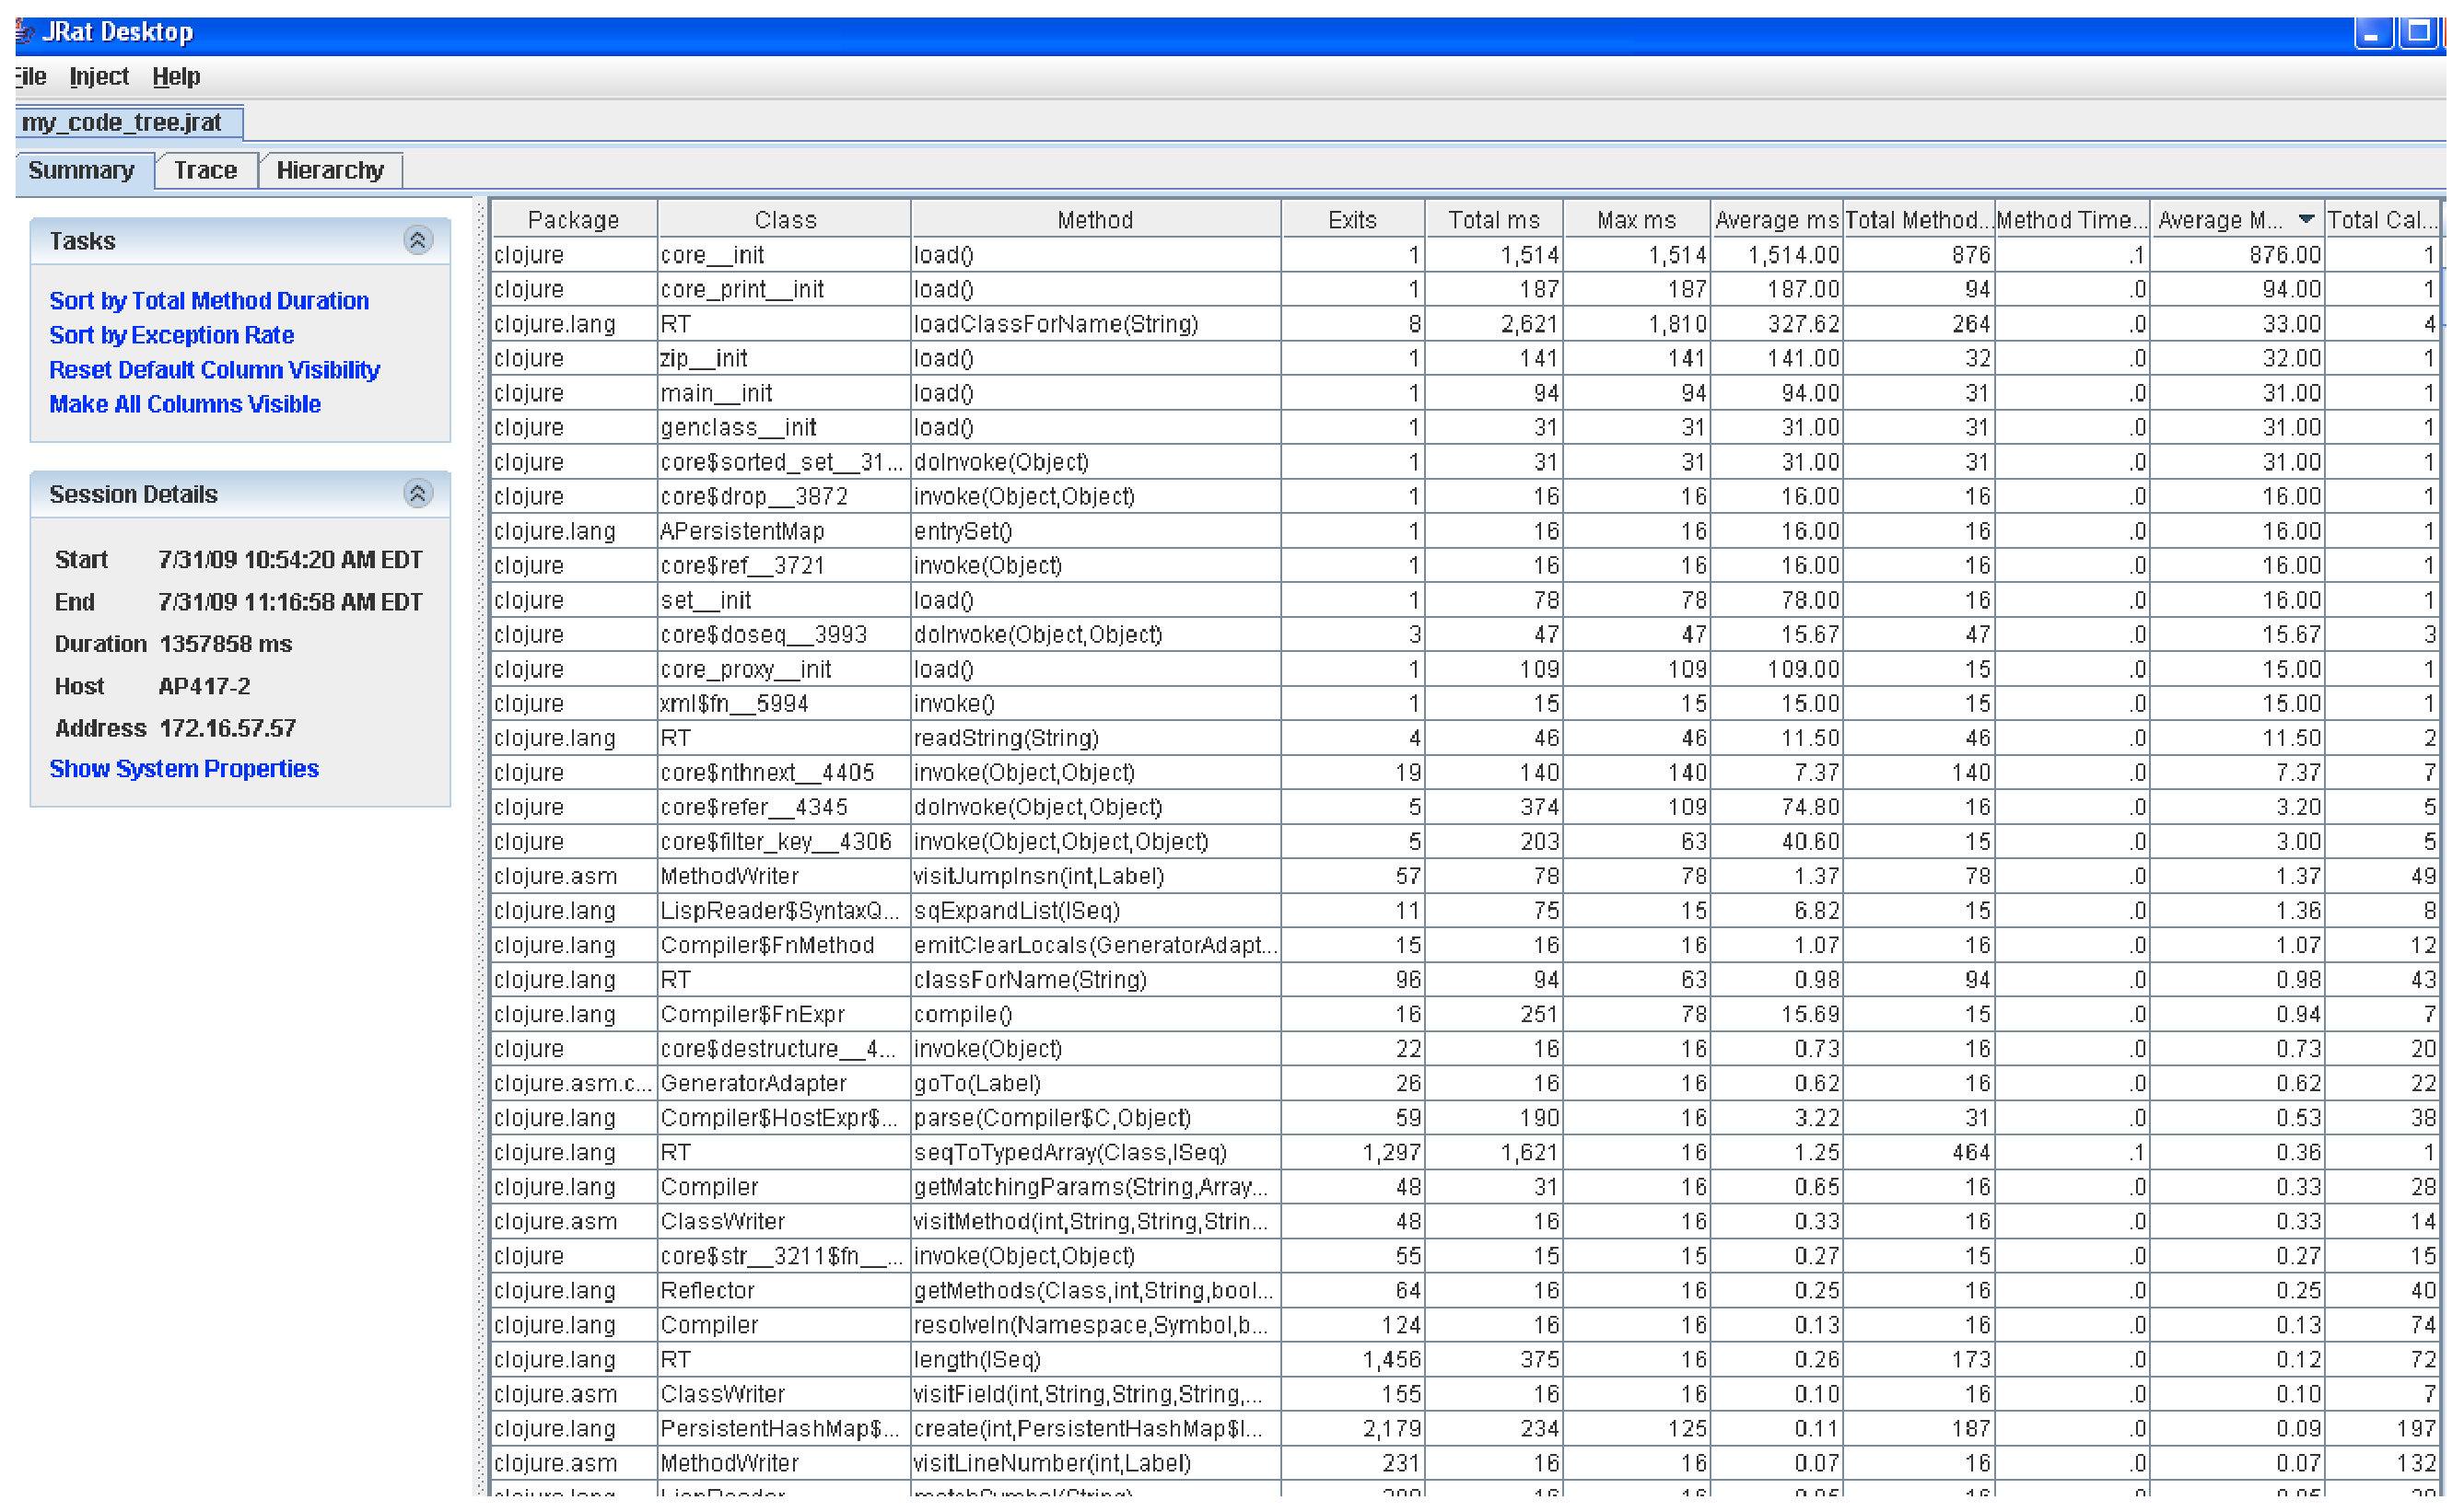
\includegraphics[width=110mm]{jrat_output_38.eps}

The screenshot above contains the jrat output after running the Clojure mandelbrot shootout application. I didn't want to analyze the results but there are a couple of stats worth taking a quick look at. The clojure.lang.Numbers.lt method had 87 million exits and a total method time of 142 milliseconds. The Numbers.ops method was called 367 million times.

The netbeans profiler contains similar profiling statistics as the jrat tool but the Netbeans profiler contains live, realtime results and a host of other metrics.

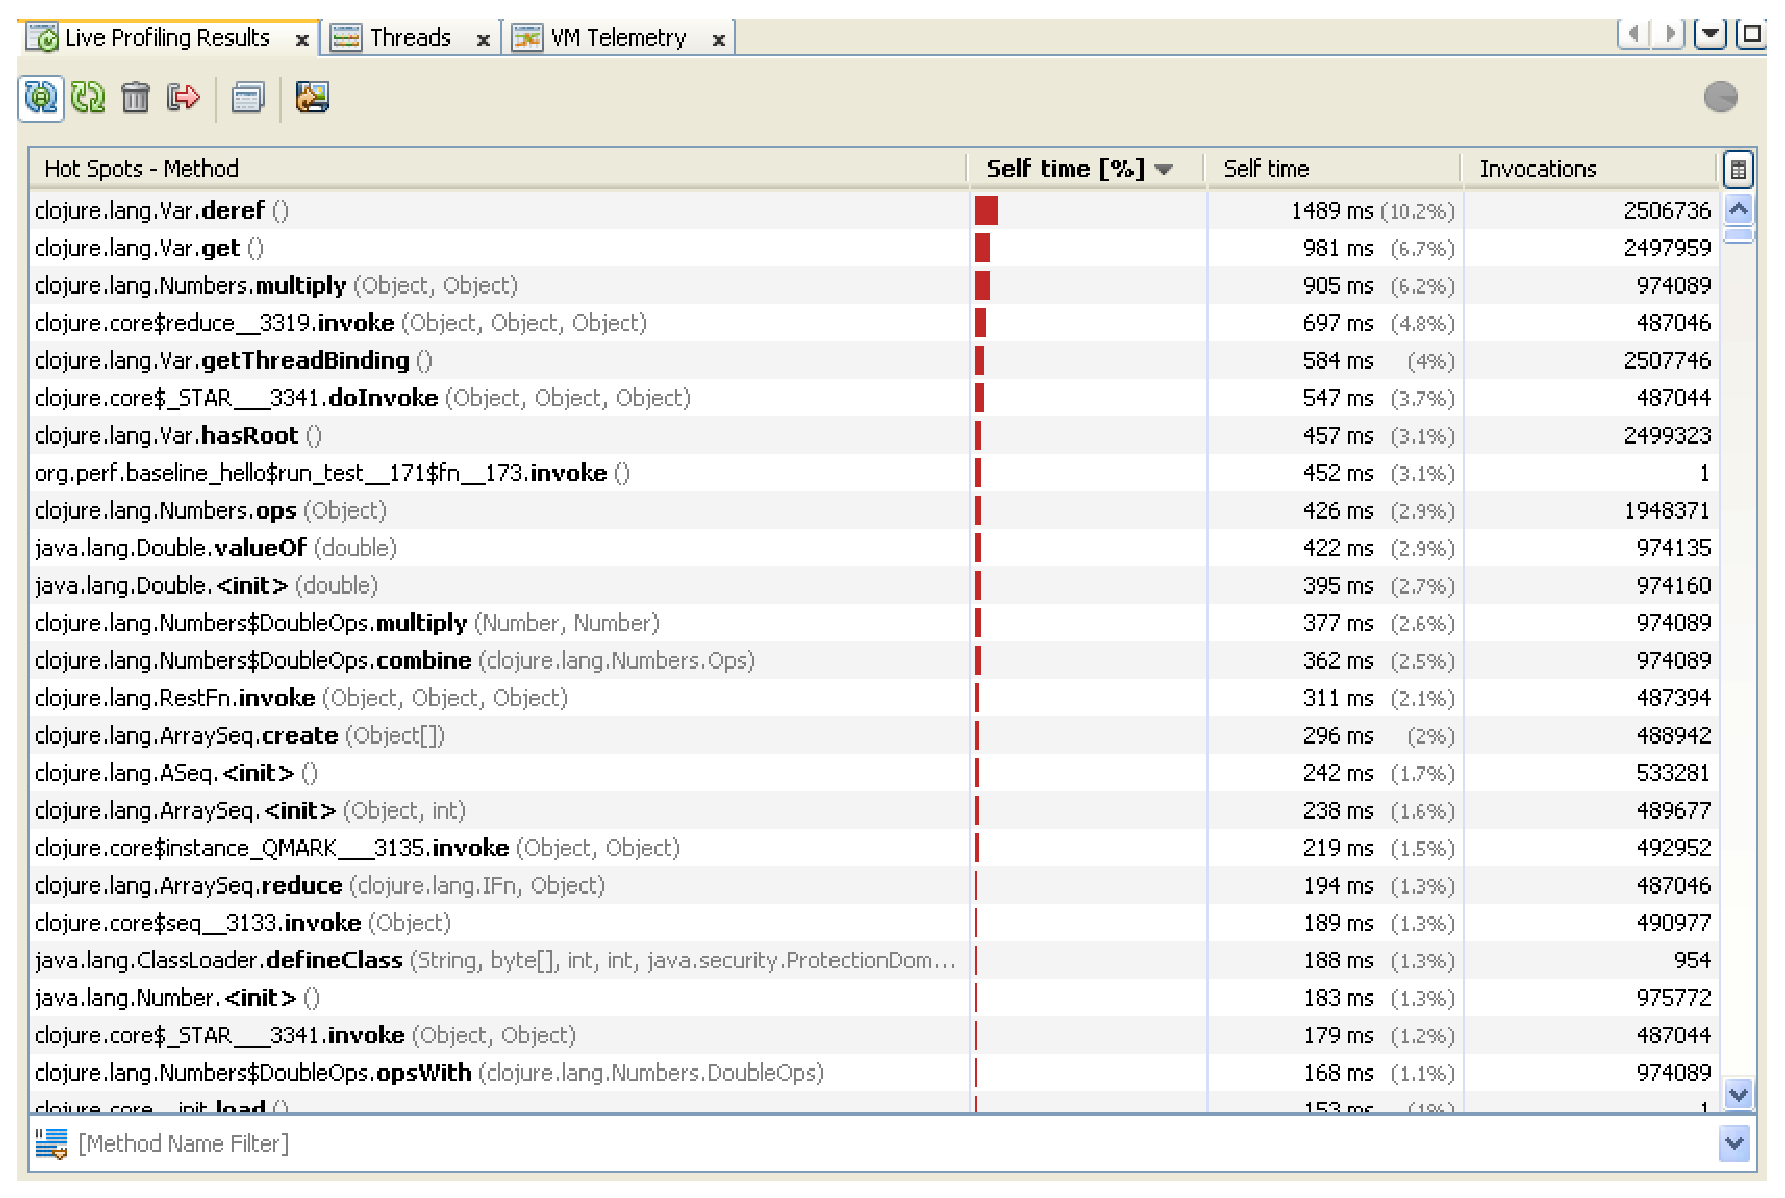
\includegraphics[width=110mm]{netbeans_profile1_40.eps}

\subsection{Testing Environment}

For this document, all of the tests were run with Java 5. Java 2 Runtime Environment, Standard Edition (build 1.5.0 11 b03)). Some tests were run with both the client and server options. The majority of tests were run with the client option. Headius describes the -server option, "The server option turns on the optimizing JIT along with a few other "server-class" settings.". Updates to the this document will include tests with Java 6.
\begin{verbatim}
* Java: Java(TM) 2 Runtime Environment Standard Edition (build 1.5.0 11 b03)
* Windows: Windows XP Professional Service Pack 2
* Hardware: Intel Core 2 CPU 6300 - 1.86ghZ, 3.49 GB of RAM

* Clojure: 1.0.0 (2009-05-04)
* JRuby: 1.3.1 (2009-06-15; 44 days ago)
* Scala: 2.7.5 (2009-06-03; 50 days ago)
\end{verbatim}
